\chapter{Results} \label{study_results}

This Chapter describes all the results gathered throughout the study in a per RQ basis. This approach increase the traceability of the findings within the report as suggested by Runeson et al. \cite{case_study_software_engineering} (Item 20 in Appendix \ref{checklist_for_case_studies}).

Furthermore, to further increase the traceability of concepts from Research questions to results these are presented in a per-research question base with distinction between quantitative and qualitative data.

As a final note, due to confidentiality issues it was not possible to report the raw data. For this reason, as briefly explained in the previous Chapter, all the sensitive information has been eliminated.

\section{Research Question 1}

Results for this Research Question are mostly quantitative. However, some of the codes generated during coding procedures are tied to the issue this particular question addresses.

\subsection{Qualitative Results}
    The coding procedures used to analyze the data that has been generated created codes that reflect bad coding practices used while developing the tests. These codes are reported in Table \inote{create table with codes and number of references.}. Furthermore, Fig. \inote{create istogram with codes divided by project} shows how these are divided among the cases under study. Finally, Tab. \inote{Create table with references of these codes}.
    

\subsection{Quantitative Results}

    As highlighted in the Related Works (section \ref{sec:related_work}), quantitative data has been extracted through static analysis of the code base. However, given the exploratory nature of this study and resources' scarcity, only few metrics have been extracted and analyzed at this stage. Figures \ref{fig:project_a_avg_complexity,fig:project_b_avg_complexity,fig:project_c_avg_complexity,fig:project_d_avg_complexity} display the results generated by the process previously described in section \ref{sec:analysis_of_the_repos}
    
\begin{figure}[H]
    \centering
    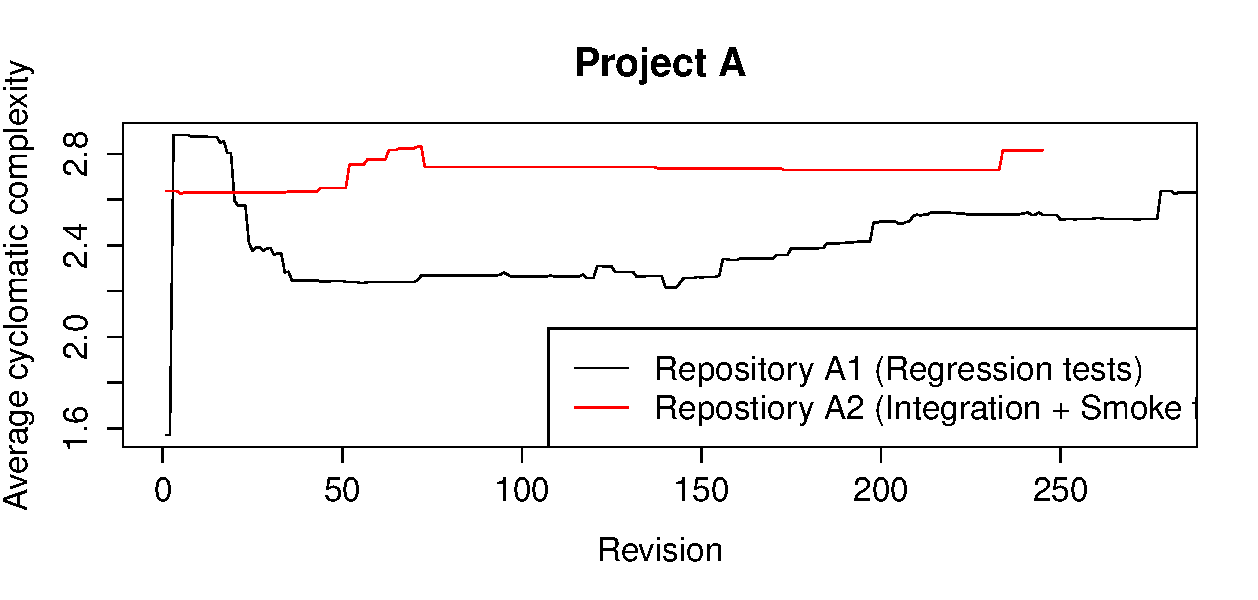
\includegraphics[width=\textwidth,keepaspectratio]{figure/results/rq1/project_a_avg_complexity.pdf}
    \caption{Project A average cyclomatic complexity over time}
    \label{fig:project_a_avg_complexity}
\end{figure}

\begin{figure}[H]
    \centering
    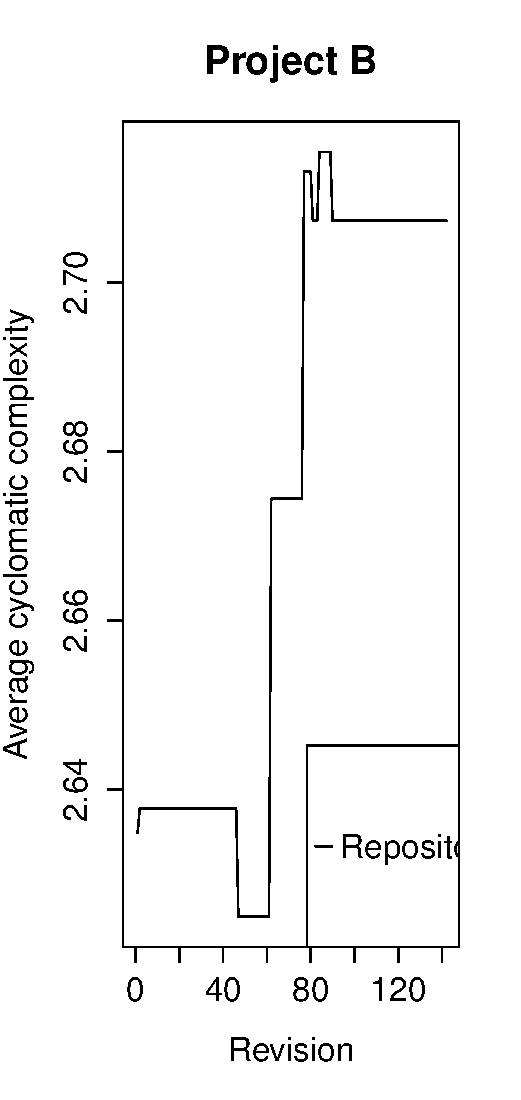
\includegraphics[width=\textwidth,keepaspectratio]{figure/results/rq1/project_b_avg_complexity.pdf}
    \caption{Project B average cyclomatic complexity over time}
    \label{fig:project_b_avg_complexity}
\end{figure}

\begin{figure}[H]
    \centering
    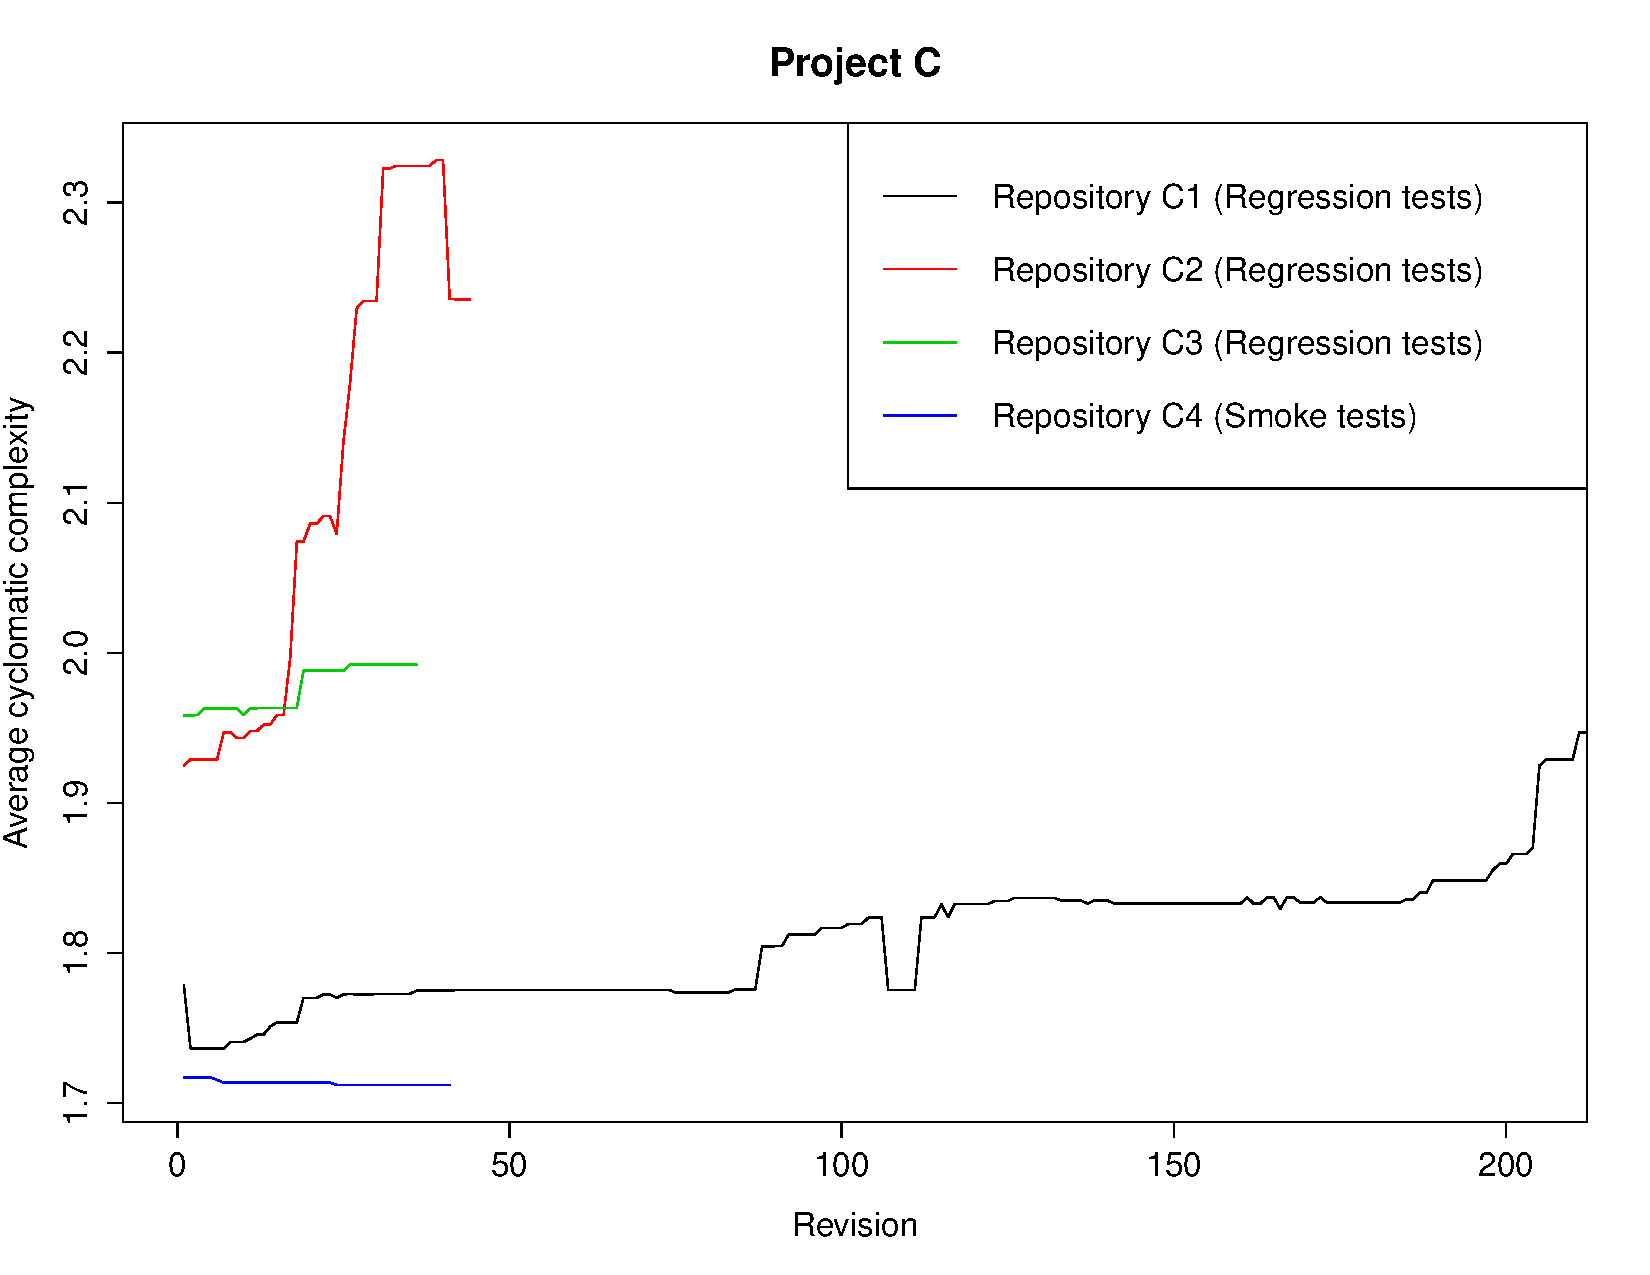
\includegraphics[width=\textwidth,keepaspectratio]{figure/results/rq1/project_c_avg_complexity.pdf}
    \caption{Project C average cyclomatic complexity over time}
    \label{fig:project_c_avg_complexity}
\end{figure}

\begin{figure}[H]
    \centering
    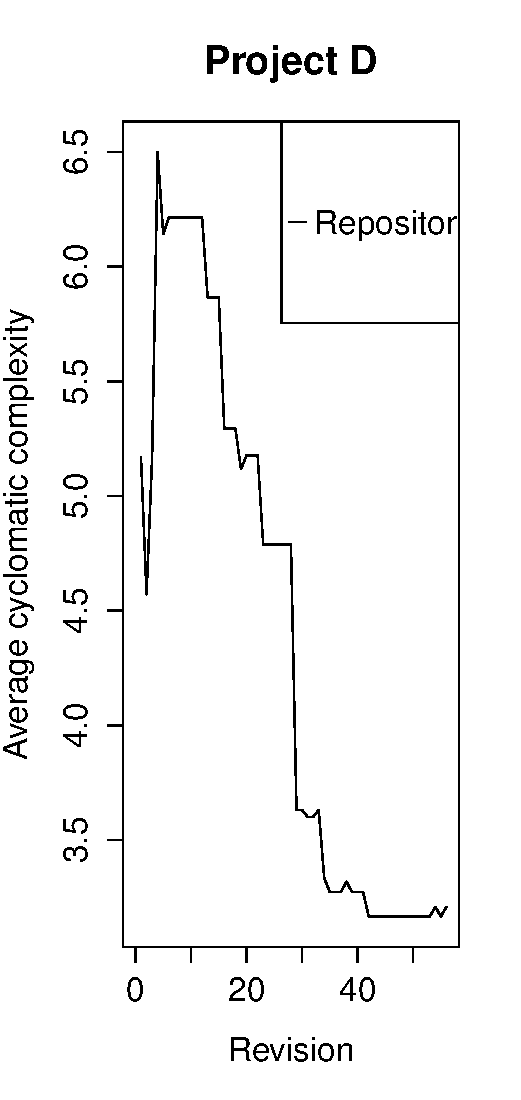
\includegraphics[width=\textwidth,keepaspectratio]{figure/results/rq1/project_d_avg_complexity.pdf}
    \caption{Project D average cyclomatic complexity over time}
    \label{fig:project_d_avg_complexity}
\end{figure}




\section{Research Question 2}

The scope of User Interface tests is to validate the state of the User Interface after a predefined series of actions occurred. However, this entails a different use for the constructs compared to conventional source code and possibly new ones specific for these use cases. For this reason the second RQ will inspect these unique items.

However, keeping into account the differences between property based testing and image recognition testing is important. The former uses property or meta-properties of UI components to identify them and simulate user events over them. The latter, instead, uses image recognition algorithms to identify such widgets. This different identification method imposes different approached when creating the test suite that are analyzed separately in the following sections, presenting both quantitative and qualitative results.

\todo{Talk about the coordinates based approach}

\subsection{Property-based problems}
    
    

\subsection{Coordinate-based problems}

\subsection{Image-recognition problems}


\section{Research Question 3}

Finally, the purpose of this RQ is to complete the description of the TD items identified by RQ 1 and RQ 2. Once again, qualitative and quantitative data has been treated separately.

\subsection{Qualitative Data}
    

\subsection{Quantitative Data}
    

